%%% -*-LaTeX-*-

\chapter{Implemention Details}

This chapter examines the implementation and encoding decisions.

\section{Language Implementation: Decisions and Alternatives}

SweetPea is an embedded domain specific language, meaning that instead of providing its own syntax and the compiler infrastructure to match, it is instead implemented as a library in an embedding language. Here we look at the choice of embedding language, as well as some choices about boolean encodings.

\subsection{Embedding Language}

The current implementation of SweetPea is embedded in Python; the syntax presented in the example code snippets in chapter 4 are valid python program snippets. The subsystem for handling Tsietin transforms is currently implemented in Haskell; an earlier implementation of the user-facing SweetPea syntax was also implemented in Haskell. We chose Haskell as an implementation language because its strong static types and functional purity lent it to verifying the correctness of the system. However, many scientists are familiar with Python, and not with Haskell syntax, so we decided to port the user-facing interface to Python to make it easier for them to use and interface with their existing workflows.

\section{Communicating with the SAT-Sampler}

\figref{fig_architecture} illustrates SweetPea's current architecture. It is more complicated than a single executable. This is partially because part of the constraints are generated by a Python program and part by the Haskell subsystem, and partially because the SAT sampler that SweetPea calls out to, Unigen, only runs on POSIX compliant systems (Linux, but not MacOS). Because of both of these facts, SweetPea is a python program which runs, and calls out to, a docker container. This docker container consists of the Haskell subsystem which can efficiently encode counting constraints, and unigen, which takes the constraints that the program compiled to and produce a satisfying assignment, should one exist.

\begin{figure}[t]
    \centerline{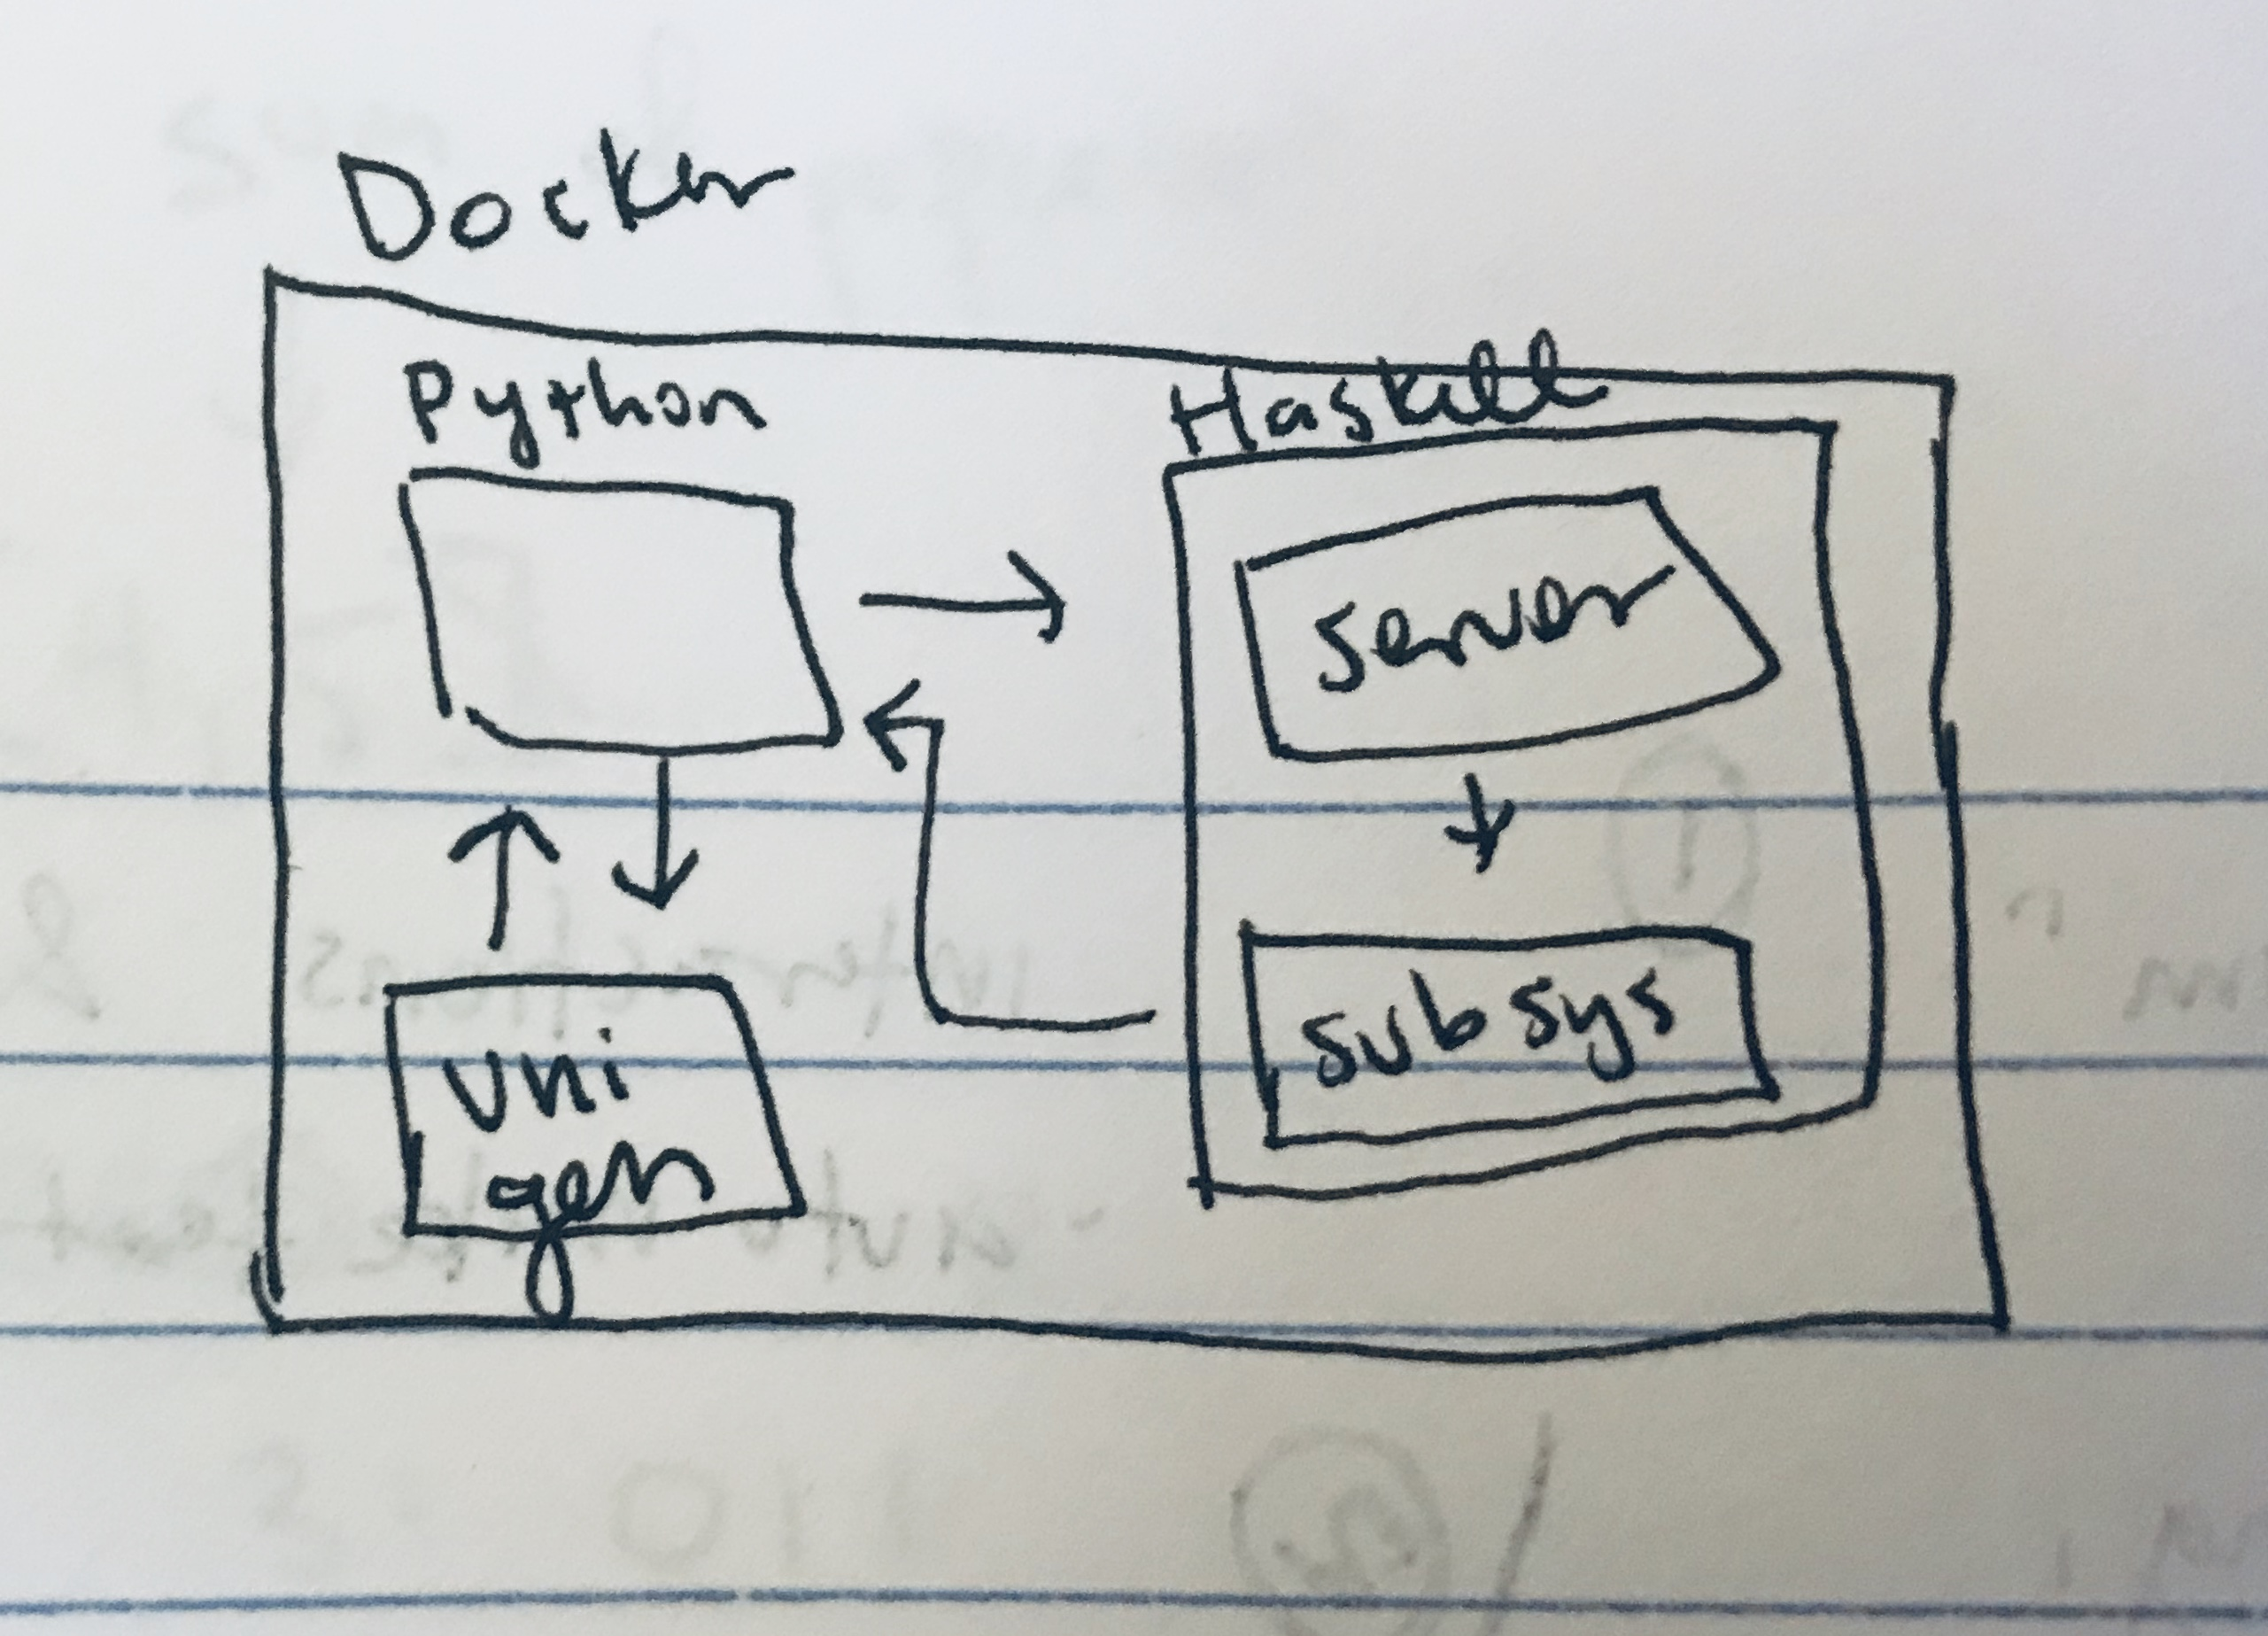
\includegraphics[origin=c,width=7cm]{fig_architecture}}
    \caption{Architecture of SweetPea deployment.}%
    \label{fig:fig_architecture}%
\end{figure}

Unigen provides two features in addition to the standard DIMACS format: the ability to denote which variables are "important" for a final assignment (in our case, those that directly encode the state of the experimental sequence), and the ability to provide xors rather than or clauses. The current version of SweetPea uses the first feature (the important variables are called the \emph{supports}), and does not use the second, though it is an optimization for future work.

After SweetPea, the python program which called out to the docker container, gets a response from unigen, it translates it back to a human-readable format. This means translating the assignments to the experimental sequence they represent (see \figref{example_assignment} for an example). The resulting sequence can either be printed as a list of strings, or can be exported to a list of python dictionaries to be directly integrated into other psychology computational tools such as psyNeuLink.

\subsection{Internal Representations}

As mentioned in the previous chapter, we encode levels by allocating one boolean variable per level to indicate the whether that level is in a selected or unselected state. This isn't the only possible


- pros / cons of using one-hot vs binary : trade-off between more variables and more clauses

- todo: more examples

\section{Encoding Counting Constraints: Tsietin Transform}
- necessary to efficeintly encode on the scale of 60 of these 120 boolean vars need to be true

- how efficient is it?

- works by mimicing popcount circuitry

- generates a bunch of "junk variables"

\subsection{Binding Variables: Iff}
- new variable "equals" if their values are in lockstep

\subsection{Adders}
- half adder example

- full adder example

\subsection{Ripple Carry Adders}
- multiple options here, the one I went with

- trade-offs of options

\subsection{Pop Count Circuit}
- pop count circuit example



\subsection{Exhaustive Testing}

- example of input / output: see how it's prone to error

- tested for a given size all assignments
